%++++++++++++++++++++++++++++++++++++++++
% Don't modify this section unless you know what you're doing!
\documentclass[letterpaper,12pt]{article}
\usepackage{tabularx} % extra features for tabular environment
\usepackage{amsmath,amsthm,amssymb,amsfonts}  % improve math presentation
\usepackage{graphicx} % takes care of graphic including machinery
\usepackage[margin=1in,letterpaper]{geometry} % decreases margins
\usepackage{cite} % takes care of citations
\usepackage[final]{hyperref} % adds hyper links inside the generated pdf file
\hypersetup{
	colorlinks=true,       % false: boxed links; true: colored links
	linkcolor=blue,        % color of internal links
	citecolor=blue,        % color of links to bibliography
	filecolor=magenta,     % color of file links
	urlcolor=blue         
}
%++++++++++++++++++++++++++++++++++++++++

%Blackboard Letters

\newcommand{\R}{\ensuremath{\mathbb{R}}}
\newcommand{\C}{\ensuremath{\mathbb{C}}}
\newcommand{\Z}{\ensuremath{\mathbb{Z}}}
\newcommand{\E}{\ensuremath{\mathbb{E}}}
\newcommand{\Prob}{\ensuremath{\mathbb{P}}}
\newcommand{\Q}{\mathbb{Q}}
\newcommand{\N}{\mathbb{N}}
\newcommand{\F}{\mathbb{F}}
\newcommand{\W}{\mathbb{W}}

%Differential d
\newcommand*{\diff}{\mathop{}\!\mathrm{d}}

% Theorem / Lemmas et cetera

\newtheorem{thm}{Theorem}[section]
\newtheorem{conj}[thm]{Conjecture}
\newtheorem{cor}[thm]{Corollary}
\newtheorem{lem}[thm]{Lemma}
\newtheorem{prop}[thm]{Proposition}
\newtheorem{exa}[thm]{Example}
\newtheorem{defi}[thm]{Definition}
\newtheorem{exe}[thm]{Exercise}
\newtheorem{rek}[thm]{Remark}
\newtheorem{que}[thm]{Question}
\newtheorem{prob}[thm]{Problem}
\newtheorem{cla}[thm]{Claim}
 
\newenvironment{problem}[2][Problem]{\begin{trivlist}
\item[\hskip \labelsep {\bfseries #1}\hskip \labelsep {\bfseries #2.}]}{\end{trivlist}}


\begin{document}

\title{C1 Assignment 3 Report}
\author{1104630}
\date{\today}
\maketitle

\begin{abstract}

\end{abstract}


\section{Theory}

The Lorenz system is the system of equations
\begin{align*}
\frac{\diff x}{\diff t} &= \sigma(y - x) \\
\frac{\diff y}{\diff t} &= x(\rho - z) - y \\
\frac{\diff z}{\diff t} &= xy -\beta z \\
\end{align*}

where $ \sigma, \rho, \beta \in \R $ are given parameters. In this assignment, we use the values originally specified by Lorenz,
\[
\sigma = 10 \text{,   } \beta = \frac{8}{3} \text{,   } \rho = 28.
\]
For these values of $ \sigma, \rho, \beta$, the system exhibits chaotic behaviour.

\subsection{Schemes}

We solve this ODE numerically using the Forward Euler method, the Runge-Kutta 4 method and the Modified Midpoint. These have global errors of order $O(h^1)$, $O(h^4)$ and $O(h^2)$ respectively.

\section{Implementation}

Rather than using the code from the last assignment, we have extensively used the ODEint library using three explicit schemes detailed above.

\section{Results}

Using the method of manufactured solutions, we calculated the $L^{\infty}$-error for the various solutions.

\subsection{Forward-Euler} 

For the Forward Euler method, we tested the implementation for $\tau = 0.001, 0.0005, 0.00025$ and $0.000125$. These were smaller time steps than for the Runge-Kutta 4 method as the order of the error is greater than for the other schemes tested. As there is no analytic solution to the ODE, we use the method of manufactured solutions to calculate the error.

\centerline{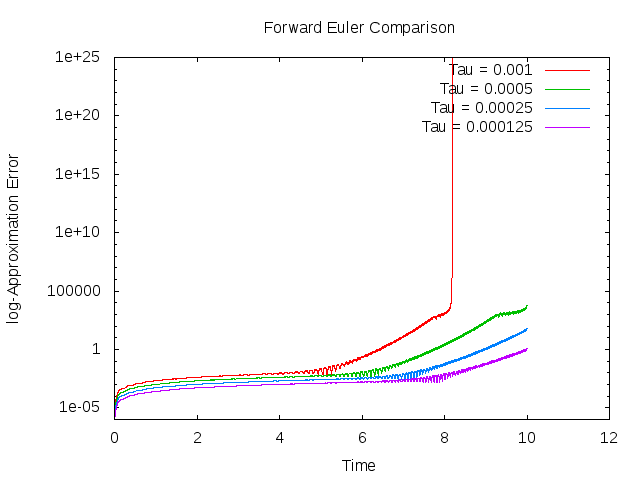
\includegraphics[scale = 0.75]{FE.png}}

As we expected reducing the time step leads to decreased error.


\subsection{Runge-Kutta 4}

For the Runge-Kutta 4 method, we tested the implementation for $\tau = 0.01, 0.005, 0.0025$ and $0.00125$.

\centerline{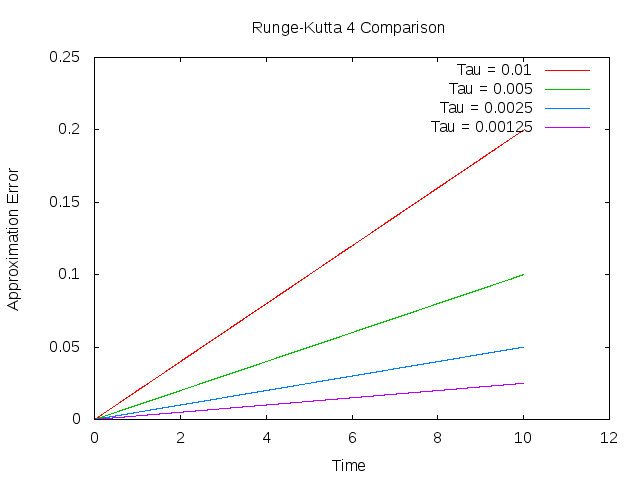
\includegraphics[scale = 0.75]{RK4.png}}

As we expected reducing the time step leads to decreased error.


\subsection{Midpoint}

For the Modified Midpoint method, we tested the implementation for $\tau = 0.01, 0.005, 0.0025$ and $0.00125$.

\centerline{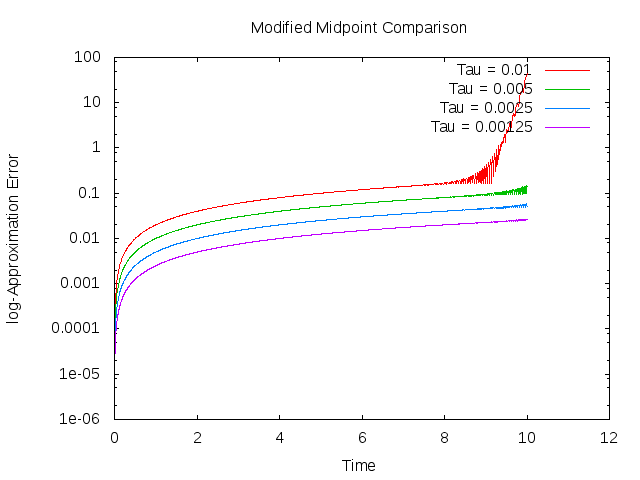
\includegraphics[scale = 0.75]{MM.png}}

As we expected reducing the time step leads to decreased error.

\end{document}
